\begin{center}
            \begin{tikzcd}[column sep =1.4cm, row sep=1.4cm]
                C \arrow[d,"f"]
                \\
                D
            \end{tikzcd}
            \hspace{0.6cm}
            \begin{tikzcd}[column sep =1.4cm, row sep=1.4cm]
                \hom(A, C)
                \arrow[r, "\eta_C"]
                \arrow[d, swap, "{f \circ(-)}"]
                &
                \hom(B, C)
                \arrow[d, "{f \circ (-)}"]
                \\
                \hom(A, D)
                \arrow[r, swap, "\eta_D"]
                &
                \hom(B, D)
            \end{tikzcd}
            \hspace{0.3cm}
            \begin{tikzcd}[column sep =0.8cm, row sep=1.4cm]
                k:A\to C
                \arrow[maps to, r, ]
                \arrow[maps to, d, swap, ]
                &
                \eta_C(k): B \to C
                \arrow[maps to, d]
                \\
                f \circ k: A  \to D
                \arrow[maps to, r, swap]
                &
                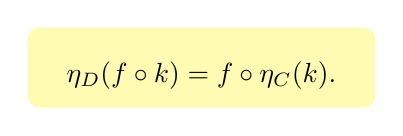
\begin{tikzpicture}
                    \filldraw[yellow!30, rounded corners] (-2.2, -0.4) rectangle (2.2,0.6);
                    \node at (0,0){$\eta_D(f \circ k)
                    =
                    f \circ \eta_C(k)$.};
                \end{tikzpicture}
            \end{tikzcd}
        \end{center}